\textit{Portions of this chapter were originally published in collaboration with Jake VanderPlas in the September 2018 edition of the Journal of Open Source Software (Fleming and VanderPlas 2018, JOSS, Vol. 3, 29, p. 781; 2018, DOI: 10.21105/joss.00781), and are reproduced below with permission of the Journal of Open Source Software. XXX - add similar text for ApJ paper}

\section{\approxposterior}

\approxposterior is a Python package for efficient approximate Bayesian inference and Bayesian optimization of computationally-expensive models. \approxposterior trains a Gaussian process (GP) surrogate for the computationally-expensive model and employs an active learning approach to iteratively improve the GPs predictive performance while minimizing the number of calls to the expensive model required to generate the GP's training set.

\approxposterior implements both the Bayesian Active Learning for Posterior Estimation (BAPE, \citet{Kandasamy2017}) and Adaptive Gaussian process approximation for Bayesian inference with expensive likelihood functions (AGP, \citet{Wang2018}) algorithms for estimating posterior probability distributions for use with inference problems with computationally-expensive models. In such situations, the goal is to infer posterior probability distributions for model parameters, given some data, with the additional constraint of minimizing the number of forward model evaluations given the model's assumed large computational cost. \approxposterior trains a Gaussian Process (GP) surrogate model for the likelihood evaluation by modeling the covariances in logprobability (logprior + loglikelihood) space. \approxposterior then uses this GP within an MCMC sampler for each likelihood evaluation to perform the inference. \approxposterior iteratively improves the GP's predictive performance by leveraging the inherent uncertainty in the GP's predictions to identify high-likelihood regions in parameter space where the GP is uncertain. \approxposterior then evaluates the forward model at these points to expand the training set in relevant regions of parameter space, re-training the GP to maximize its predictive ability while minimizing the size of the training set. Check out the BAPE paper by \citet{Kandasamy2017} and the AGP paper by \citet{Wang2018} for in-depth descriptions of the respective algorithms.

\approxposterior is an implementation of the ``Bayesian Active Posterior Estimation" (BAPE) algorithm developed by \citet{Kandasamy2017}, but with several modifications to afford the user more control over the inference. Below, we qualitatively describe this algorithm, define parameters, and suggest typical values. We then discuss \approxposterior's convergence scheme.

\section{\approxposterior Algorithm} \label{AP:sec:app}

Qualitatively, the \approxposterior algorithm is as follows. First, assume a forward model with $d$ input parameters that is designed to reproduce some set of observations. In our case, $d$, the dimensionality of parameter space, is five. The model parameters have an input domain, $D$, that is defined by the user. The parameters are further described by a prior probability distribution based on the user's prior belief for how the model parameters are distributed.  Next, the user generates a training set, $T$, consisting of $m_0$ forward model simulations distributed across the parameter space. The user chooses how the $m_0$ samples are distributed throughout parameter space according to their preferred experimental design. \approxposterior then trains a GP on $T$ to construct a non-parametric model (sometimes called a ``surrogate model") that represents the outcomes of the forward model over the parameter space. Crucially, GPs also generate an uncertainty for the surrogate model at every point in parameter space.

\approxposterior then identifies $m$ more locations in parameter space to apply the forward model and add to $T$. The new locations are selected by determining the regions that the GP has identified as having both a high lnprobability, i.e. high posterior density, and a high predictive uncertainty. This selection is accomplished by maximizing a utility function ($u$, described below) that quantifies where the GP predicts high posterior density and high uncertainty in parameter space, focusing resources on parameter combinations that are likely to be consistent with the observations. \approxposterior re-trains the GP with the augmented $T$. The GP is then passed to an MCMC algorithm, e.g. \emcee, that samples the parameter space to obtain the approximate posterior distributions of the model parameters.

At the end of each iteration, \approxposterior checks if a convergence condition (described in $\S$~\ref{AP:sec:app:convergence}) has been met. If the algorithm  has not yet converged, \approxposterior selects an additional $m$ new points to add to $T$, re-trains the GP, and again estimates the posterior distribution. This process repeats until convergence or until \approxposterior has run the maximum number of iterations, $n_{max}$, set by the user. In Algorithm~\ref{AP:app:algo}, we list the aforementioned steps that comprise this algorithm.

\begin{algorithm} 
\SetAlgoLined
 Assume an input domain $D$, GP prior on $f(\textbf{x})$ \\
 Generate a training set, $T$, consisting of $m_0$ pairs of $(\textbf{x}, f(\textbf{x}))$ \\
 \For{$t=0, 1, ..., n_{\mathrm{max}}$}{
    \For{$i=0, 1, ..., m$}{
      Find \textbf{x}$^+$ = argmax$_{\textbf{x} \in D}$ $u(\textbf{x})$ \\
       Compute $f(\textbf{x$^+$})$ \\
       Append $(\textbf{x$^+$}, f(\textbf{x$^+$}))$ to $T$ \\
       Re-train GP, optimize GP hyperparameters given augmented $T$ \\
   }
   Use MCMC to obtain approximate posterior distribution with GP surrogate for $f(\textbf{x})$ \\
   \If{$\mathrm{converged}$}{
        \textbf{break} \\
    }
 }
\caption{\approxposterior Approximate Inference Pseudo Code  \label{AP:app:algo}}
\end{algorithm}
where $f(\textbf{x}) = \mathcal{\ln L}(\textbf{x})$ + $\ln \mathrm{Prior}(\textbf{x})$, i.e. the lnprobability function used for MCMC sampling with \emcee and \textbf{x}$^+$ is the point in parameter space selected by maximizing $u$. For our application, evaluating $f(\textbf{x})$ requires running a \vplanet simulation to compute $\mathcal{\ln L}(\textbf{x})$ (see $\S$~\ref{trap:sec:mcmc:like}).

By placing a GP prior with a squared exponential kernel on $f(\textbf{x})$, we assume that the function is smooth and continuous, both reasonable assumptions for modeling the posterior density. For inference problems that are liable to violate these assumptions, other kernels, e.g. the Ornstein-Uhlenbeck kernel, may be more appropriate (we refer the reader to \citet{Rasmussen2006} for detailed descriptions of common GP kernels and their mathematical properties). \approxposterior uses \texttt{george} \citep{george} for all GP calculations and hence users can apply any kernels implemented in that software package.

\approxposterior has several free parameters that can be set by the user: $m_0$, the size of the initial training set (50 in our case), $n_{\mathrm{max}}$, the maximum number of iterations (15), $m$, the number of new points to select each iteration where the forward model will be evaluated (50 per iteration), and $\epsilon$, the convergence threshold (0.1). Typically, we find that $n_{\mathrm{max}}=2-3 \times d$, $m, m_0 = 10-20 \times d$, and $\epsilon = 0.1$ work well in practice, although performance may vary depending on the use case. For a complete list of \approxposterior parameters, we refer the reader to the online documentation.\footnote{ \href{https://dflemin3.github.io/approxposterior}{https://dflemin3.github.io/approxposterior/}}

Note that \approxposterior does not linearly transform the parameter space to the unit hypercube as did \citet{Kandasamy2017}. Moreover, \approxposterior does not fix the covariance scale lengths, instead opting to estimate all GP kernel hyperparameters by maximizing the marginal likelihood of the GP, given its training set, at a user-specified cadence. In Algorithm~\ref{AP:app:algo}, we optimize the GP hyperparameters each time a new point is added to the training set, but in practice we found this is unnecessary, especially at later iterations when the GP has developed a reasonable approximation of the posterior. The authors prefer to optimize the GP hyperparameters twice per iteration, once after half of the $m$ new points have been selected, and again after all $m$ points have been selected.

\section{Augmenting the Training Set} \label{AP:sec:augment}

Each iteration, \approxposterior selects $m$ new points to add to the GP's training set by maximizing the utility function, $u$. To motivate the choice of $u$, consider the following argument based on \citet{Kandasamy2017}: \approxposterior assumes that the forward model the GP learns on, here \vplanet via $\ln \mathcal{L}$, is computationally-expensive to run, and hence \approxposterior seeks to minimize the number of forward model evaluations required to build its training set. For inference problems, it is natural to select high-lnprobability regions in parameter space to augment the GP training set as this is where the posterior density is large. Furthermore, selecting regions in parameter space where the GP's predictive uncertainty is already small offers little value, compared to regions where its predictions are more uncertain, as additional points in low-uncertainty regions are unlikely to alter the GP's predictions. 

With these considerations in mind, \citet{Kandasamy2017} leverage the analytic properties of GPs to derive the ``exponentiated variance" utility function, given by their Eq.~(5)
\begin{equation} \label{AP:eq:bape}
    u_{\textrm{EV}}(\textbf{x}) = \exp(2 \mu_t(\textbf{x}) + \sigma_t^2(\textbf{x}))(\exp(\sigma_t^2(\textbf{x})) - 1),
\end{equation}
where $\mu_t(\textbf{x})$ and $\sigma_t^2(\textbf{x})$ are the mean and variance of the GP's predictive conditional distribution evaluated at \textbf{x}, respectively, for the $t^{th}$ \approxposterior iteration. To select each point, we maximize Eqn.~\ref{AP:eq:bape} using the Nelder-Mead method \citep{Nelder1965}. Note that this optimization is rather cheap since it only requires evaluating the GP's predictive conditional distribution, so this task is not a significant computational bottleneck. We restart this optimization 5 times to reduce the influence of local extrema. Note that in practice, we optimize the natural logarithm of the utility function to ensure numerical stability.

\begin{figure}
	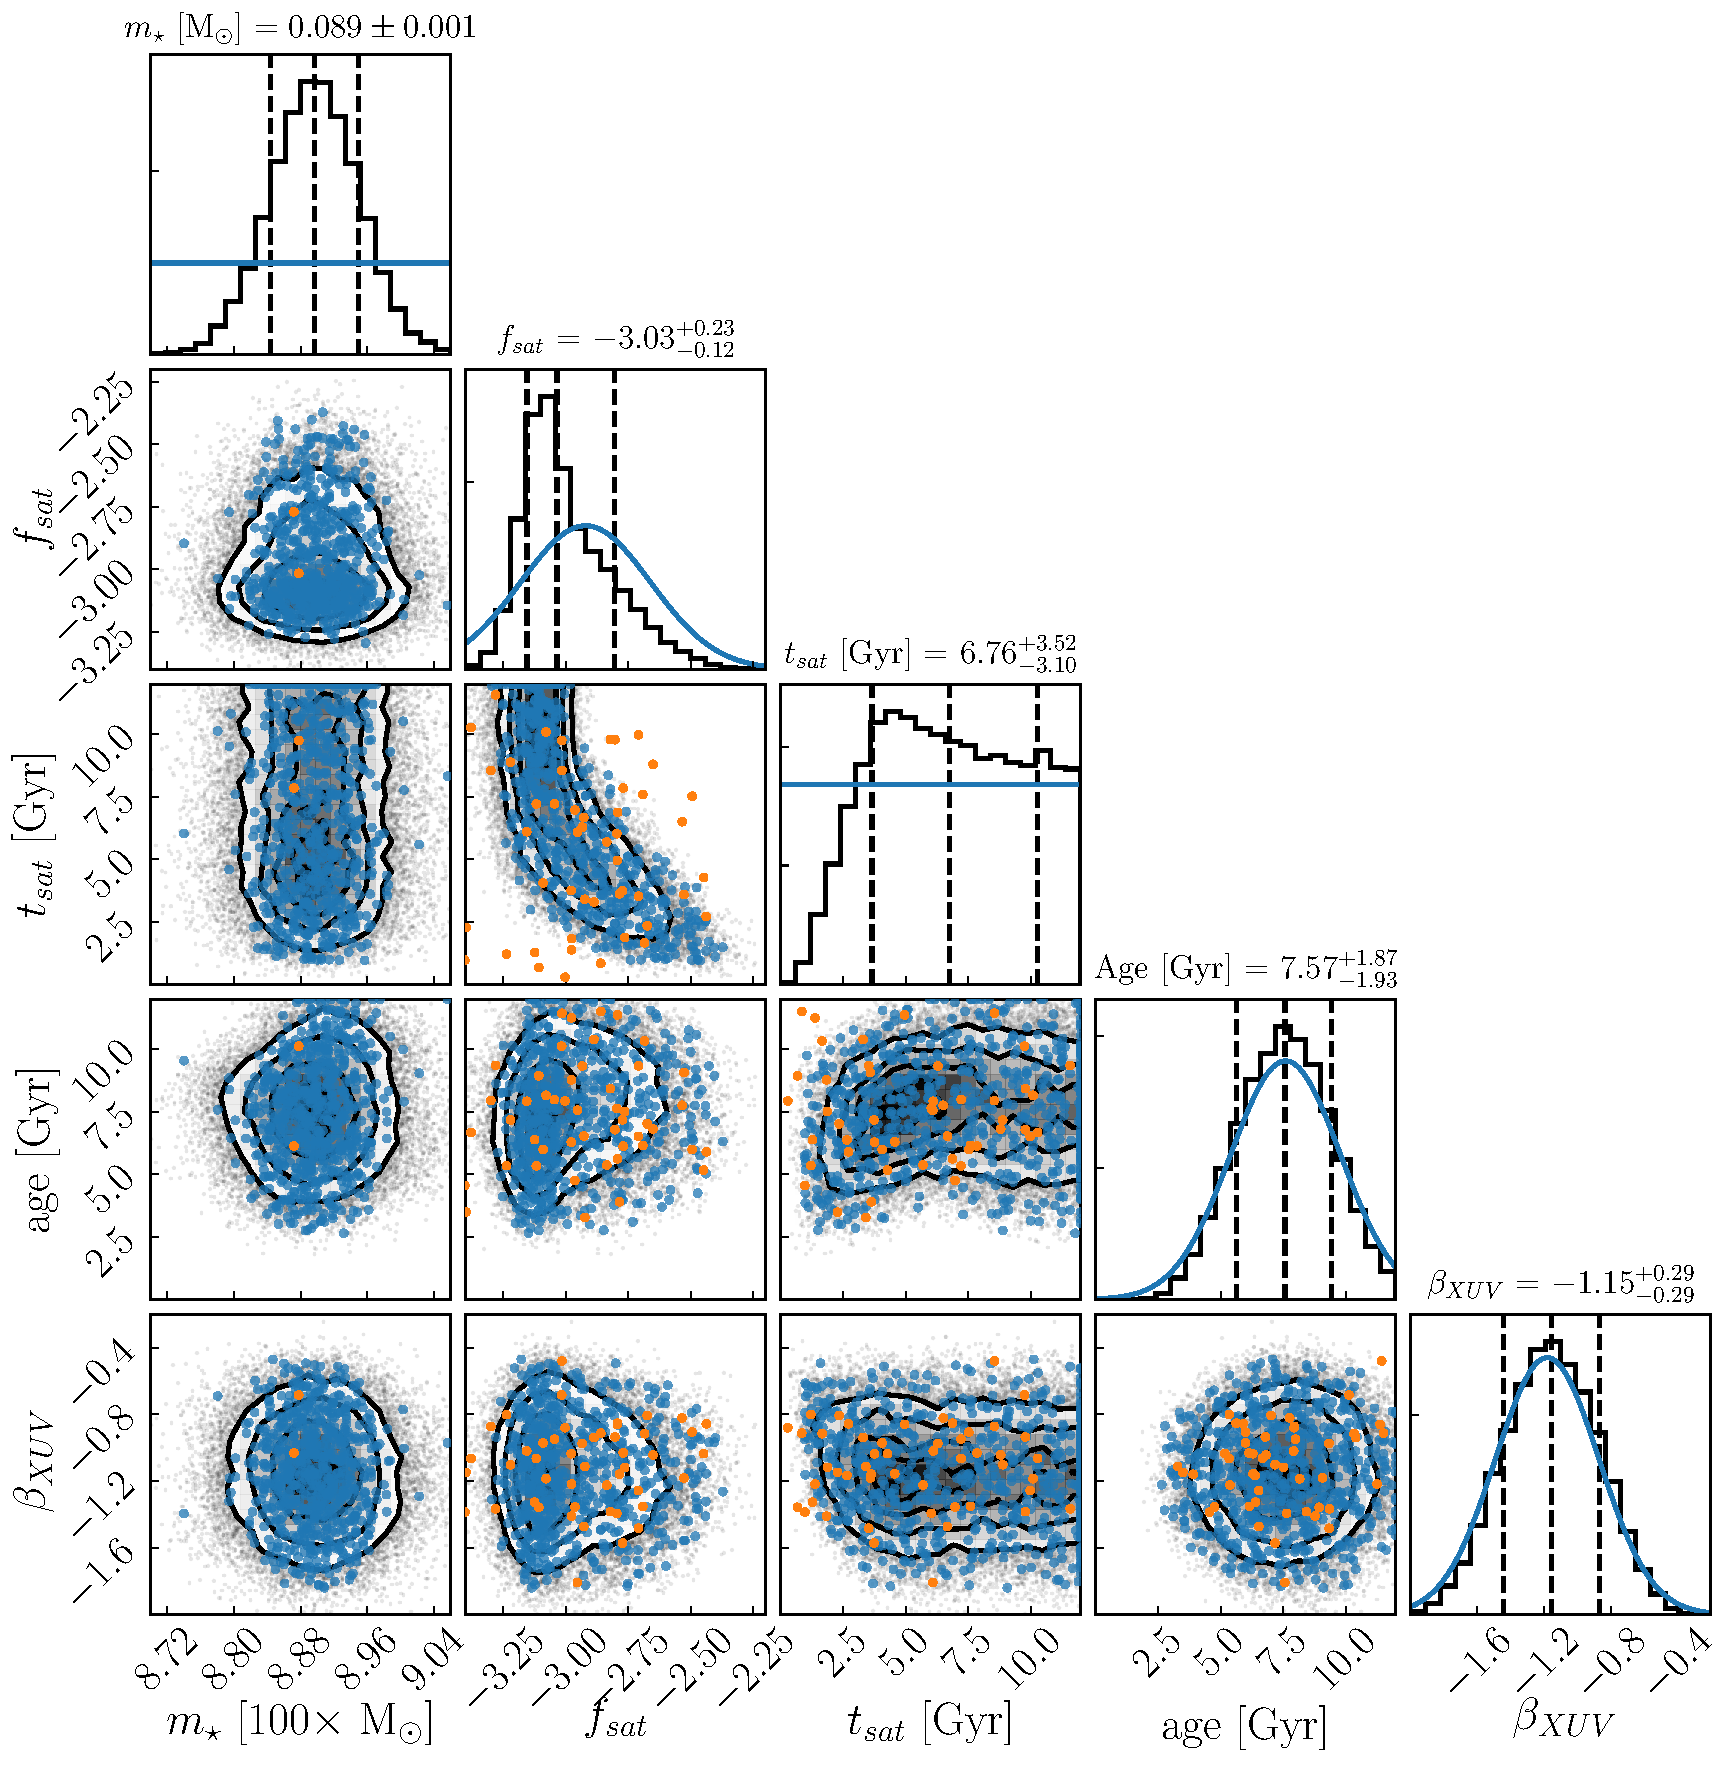
\includegraphics[width=\textwidth]{points.pdf}
   \caption{Same as Fig.~\ref{trap:fig:approx}, but overplotted with the training set for \approxposterior's GP. The orange points display the initial training points whereas the blue points display the points iteratively selected by maximizing the \citet{Kandasamy2017} utility function, Eqn.~(\ref{AP:eq:bape}). By design, \approxposterior selected points to expand its training set in regions of high posterior density, improving its GP's predictive accuracy in the most relevant regions of parameter space while seldom wasting computational resources in the low likelihood regions.}%
    \label{AP:fig:points}%
\end{figure}

As demonstrated in \citet{Kandasamy2017}, Eqn.~(\ref{AP:eq:bape}) identifies high-likelihood points where the GP's predictions are uncertain, significantly reducing the cost of training an accurate GP surrogate model. We highlight this behavior for our own application in Fig.~\ref{AP:fig:points} by displaying the approximate posterior distribution derived by \approxposterior from \citet{Fleming2020} overplotted with the initial training set in orange and the points selected by sequentially maximizing Eqn.~(\ref{AP:eq:bape}) in blue. Given the small initial training set, \approxposterior successfully selects high-posterior density points in parameter space to augment the GP's training set. Some points are selected in low-likelihood regions early on, typically near the edges of parameter space where the GP's uncertainty was initially large.

% extra
%\xxx{\citet{Wang2018} derive the entropy-based utility function (``Adaptive Gaussian Process", AGP) that is designed to select the point \textbf{x} that, when added to the GP training set $T$, maximizes the information gain for the inference problem. The \citet{Wang2018} utility function given by their Eq.~(7)}
%\begin{equation} \label{app:eq:agp}
%    u_{\textrm{AGP}}(\textbf{x}) = \mu_t(\textbf{x}) + \frac{1}{2}\ln{(2\pi e \sigma_t^2(\textbf{x}))}
%\end{equation}
%where $e$ is Euler's number.

\section{Convergence} \label{AP:sec:app:convergence}

We assess the convergence of the \approxposterior algorithm by comparing the means of the approximate marginal posterior distributions over successive iterations. We consider an \approxposterior run ``converged" if the differences between the marginal posterior means, relative to the widths of the marginal posteriors, are less than a tolerance parameter, $\epsilon$, for $k_{max}$ consecutive iterations. Effectively, this criterion checks if the expected value of each model parameter over the posterior distribution varies by ${\leq}{\epsilon}$ standard deviations from the previous iteration's expected values. That is, we require the \approxposterior convergence diagnostic $z_{t,j}{\leq}{\epsilon}$ for all $j$, where
\begin{equation}
    z_{t,j} = |\mu_{t,j} - \mu_{t-1,j}| / \sigma_{t-1,j},
\end{equation}
 and $\mu_{t,j}$ and $\sigma_{t,j}$ are the mean and standard deviation of the approximate marginal posterior distribution for the $t^{th}$ iteration and the $j^{th}$ parameter. This quantity is analogous to the ``z-score" commonly used in many statistical tests. Following \citet{Wang2018}, we require this condition to be satisfied for $k_{max}$ consecutive iterations to ensure \approxposterior is producing a consistent result. With this scheme, \approxposterior tolerates deviations from the previous estimate that are less than, or at least consistent with, the previous values, given the inherent uncertainty implied by the width of the posterior distribution. For our application, we adopted conservative choices of $\epsilon = 0.1$ and $k_{max} = 5$. Each \approxposterior iteration, we also visually inspected the estimated posterior distribution to ensure convergence. 

In Fig.~\ref{AP:fig:convergence}, we display the convergence diagnostic quantity, $z_t$, as a function of iteration for each model parameter for the \approxposterior run presented in the main text. \approxposterior quickly finds a consistent result as $z_t$ decreases below our convergence threshold within the first few iterations. For each parameter, $z_t$ continues to decrease until iteration 3 before stabilizing. The evolution of $z_t$ is not monotonic, however, owing to the stochastic nature of GPs, our hyperparameter optimization scheme, and MCMC sampling that can cause these values to occasionally be slightly worse than previous iterations. Requiring convergence over $k_{max}$ consecutive iterations mitigates the impact of this stochasticity.

\begin{figure}
\centering
	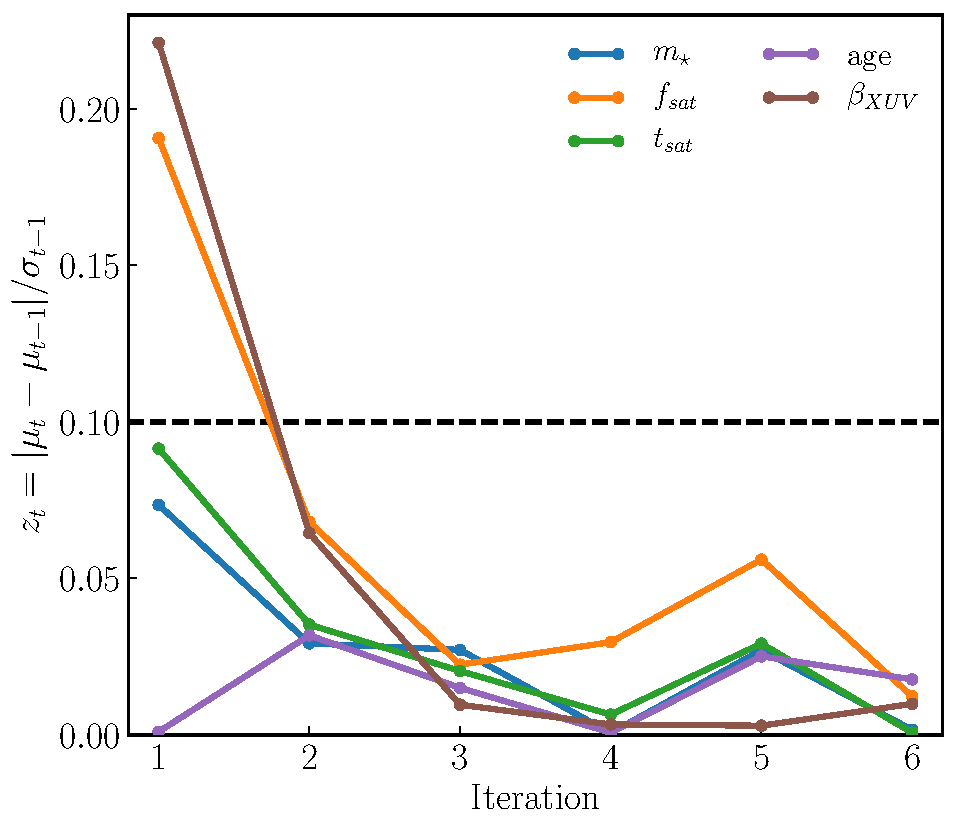
\includegraphics[width=\textwidth]{convergence.pdf}
   \caption{The \approxposterior convergence diagnostic, $z_t$, as a function of iteration for the run presented in the main text. Note that in \approxposterior, the initial iteration is iteration 0. The black dashed line indicates our adopted convergence threshold of $\epsilon = 0.1$. \textbf{\approxposterior quickly converges to a consistent and accurate result.}}%
    \label{AP:fig:convergence}%
\end{figure}